%# -*- coding: utf-8-unix -*-
%%==================================================
%% chapter02.tex for SJTU Master Thesis
%% Encoding: UTF-8
%%==================================================

\chapter{ 立体场景中的人眼视觉}
\label{chap:humanview}

\section{人眼视觉的生理过程}
\label{sec:humanvisual}

人的视觉系统是双目系统,这就决定了人眼的视觉过程既有单目线索,也有双目线索。单目线索是单只眼睛在观看过程中的生理变化,双目线索既包括单目线索的叠加信息,也存在单目线索的交叉信息。本部分将从这两个方面论述人眼视觉的生理过程,进而论证其与眼动数据之间的联系。
\subsection{人眼单目生理过程}
\label{sec:singleye}

人眼结构如图\ref{fig:eye}所示\footnote[1]{St. Luke’s Cataract and Eye institute, \url{http://www.stlukeseye.com/}},最外层部分分为角膜和巩膜两部分,其中前面1/6的区域为角膜,剩余部分为巩膜。巩膜具有维持眼球形状和保护眼内组织的功能。角膜下方的有色部分称为虹膜,虹膜围绕的区域为瞳孔。光线首先穿过透明的角膜,然后进入虹膜,再到达眼睛的更深处,此时,虹膜会牵引其附着的肌肉来调节瞳孔的大小,以控制进入眼球的光线的量。瞳孔内部是晶状体,其作用是调节眼睛肌肉,使眼睛可以分辨出所看物体的远近。
\begin{figure}[!htp]
  \centering
  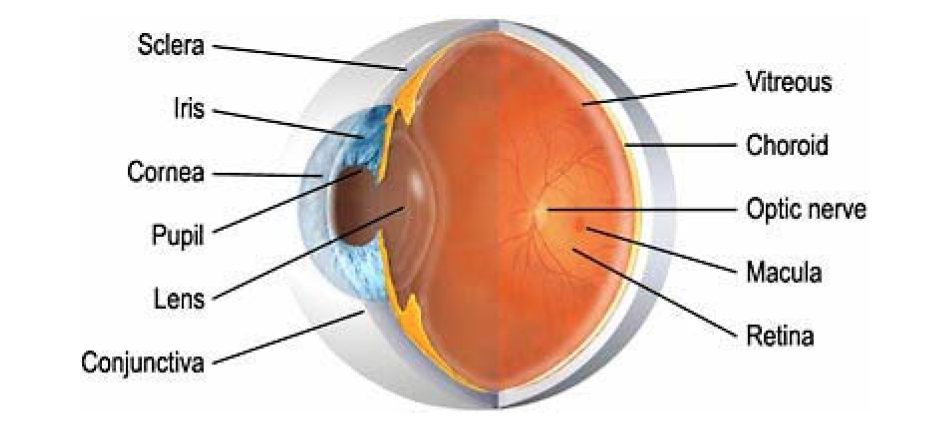
\includegraphics[width=0.6\textwidth]{chap2/eye.png}
  \bicaption[fig:eye]{人眼的生理结构示意图}{人眼的生理结构示意图\footnote[1]{St. Luke’s Cataract and Eye institute, \url{http://www.stlukeseye.com/}}}{Fig}{The human eye\footnote[1]{St. Luke’s Cataract and Eye institute, \url{http://www.stlukeseye.com/}}}
\end{figure}
当人眼观看时,会在眼睛后方的视网膜上形成一幅颠倒的图像。视网膜上包含数量众多的感光细胞----杆细胞和锥细胞,杆细胞的数量约为1亿2000万左右,它不能分辨颜色,但是可以分辨较暗的光线。锥细胞约600万,位于黄斑区内,不仅可以分辨光的强度,而且可以分辨光的颜色,其正常机理需要满足一定的光强度。黄斑中心锥细胞密度最高的区域称为中央凹,这是视网膜中最敏感的部分,人眼大部分的视觉处理是通过中央凹完成的。感光细胞将光刺激转化为电刺激并通过视神经传入大脑,在大脑中还原成所看到的图像\parencite{atchison2000optics}。

单目生理过程表明,眼睛的成像过程其实是眼睛在大脑皮层的指挥下对进入眼球的图像从亮度和色度等维度先进行分解,生成光刺激,在感光细胞的作用下,这些刺激转化为电刺激,从而传入大脑进行处理,这是基于图像特征的图像质量评价方法的生理学基础。同时可以看出,眼睛对进入眼球的信息控制是由眼部肌肉牵引相关部位完成的,也就是说,针对不同的信息,眼睛会通过相关的运动来调节处理。这表明,眼睛的运动过程是大脑对进入眼睛信息量与信息类别控制的结果。这是近年来眼动仪等科技产品被引入视觉研究领域的理论依据。
\subsection{人眼双目生理过程}
\label{sec:doubleye}

人类视觉系统的双目性表明,人眼对所处世界的观察来源于两只眼睛共同作用的结果。眼球的左右移动,使得双目几乎在所有时刻都对同一场景产生出略有差异的两幅图像,通过单目视觉系统,两幅图像首先被感知区域的神经节细胞捕捉,然后会被转移到左右外侧膝状体,最后到达大脑皮层。大脑皮层($V1$ 区域)首先接收到这些信息,这里分布着简单细胞和复杂细胞,简单细胞能够感知方向、大小以及空间频率的相位等信息,同时,为了处理来自双眼的信息,简单细胞会成对工作。而复杂细胞则可以连接两个简单细胞,以此产生双目视觉\parencite{bensalma2013perceptual}。

生理学研究成果进一步表明,简单细胞有单目简单细胞和双目简单细胞之分,同理,复杂细胞也包括单目复杂细胞和双目复杂细胞。Hubel等\parencite{hubel1962receptive}定义了简单细胞的基本概念,它被认为是反应立体视觉中边界、轮廓的关键性元素。同时,简单细胞也被用来做局部空间频率分析。Fleet等\parencite{fleet1996neural}建立了复杂细胞的模型,两个单目简单细胞与一个单目复杂细胞相连接,这两个单目细胞轮流计算同一区域的信号。而一个双目复杂细胞与两组双目简单细胞中的其中之一相连接,这两组简单细胞之间存在着一定的相位差。具体地,简单细胞与复杂细胞的关系如图\ref{fig:simplecomplexcell}所示。这是大脑皮层层次在视觉过程中的生理变化。
\begin{figure}[!htp]
  \centering
  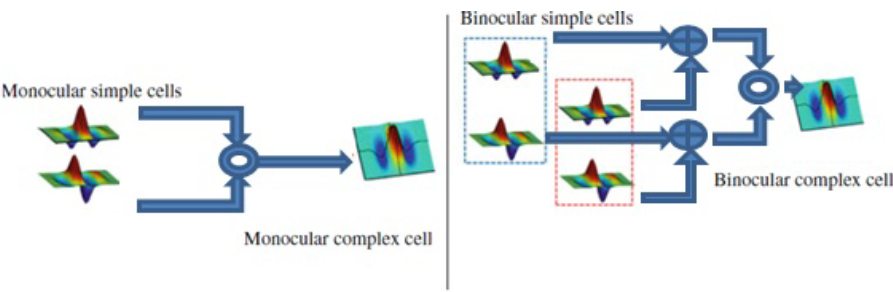
\includegraphics[width=0.8\textwidth]{chap2/simplecomplexcell.png}
  \bicaption[fig:simplecomplexcell]{简单细胞和复杂细胞之间的关系}{简单细胞和复杂细胞之间的关系\supercite{galkandage2015full}}{Fig}{Relationship between monocular and binocular, simple and complex cells\supercite{galkandage2015full}}
\end{figure}

从上述的双目融合过程可以看出,简单细胞与复杂细胞的生理特性与图像的方向、大小、相位、频率等特征相关,使得双目融合成为图像质量评价中纹理、轮廓提取、频域变化等方法的生理学基础。立足于这些生理学基础,科研人员模拟人类视觉过程建立了一系列图像质量评价模型\parencite{bensalma2013perceptual,engelke2011visual,hachicha2013stereo,ryu2014no}。同时,双目视觉过程表明了,只有进入人眼视觉系统的部分才决定了人对图像质量的判断。因此,为了提高特征提取的精度,人眼注视区域的特征也逐步替代了整体图像的特征,这也为眼动仪在图像质量评价方法中得到应用创造了条件。
\subsection{人眼视觉系统对图像视差的处理过程}
\label{sec:disparityprocess}
前面提到,人眼双目几乎在任何时候都会对同一场景产生出略有差异的两幅图像,这种差异我们用视差来描述\parencite{bensalma2013perceptual}。从几何学的角度来看,视差有水平视差和垂直视差之分(以平面正交坐标系为参考)。由于人眼是水平排列的,所以,水平视差在立体成像过程中起决定性作用。人眼对视差的处理结果形成了人类对现实世界的立体感知,这是千百年来人类进化过程中自然场景长期刺激的结果\parencite{liu2010scene}。

人眼对视差敏感的神经元分布在大脑皮层$V1$区域\parencite{hubel1962receptive},最新研究成果发现\parencite{barlow1967neural, nikara1968analysis, pettigrew1968binocular},纹状皮层上也存在着对视差敏感的神经元。研究表明,简单细胞的神经元具有视差选择性,其作用是对一定范围内的视差选择性地做出反应,并且这些细胞会对处理过的视差具有记忆性。这个事实表明,人眼并不是无限制的接纳任意大的视差,当视差超出神经元记忆的峰值之后,人眼并不会有效的对这部分信息进行处理,这与我们在后面的眼动实验中观察的结果是一致的。另外,双目的视差敏感区域并不在视网膜的同一位置,且大小也可能不一样。Anzai等\parencite{anzai1999neural}的研究成果表明,视差敏感神经元还存在相位差,且相位差在双目视差的编码中起主导作用。这也为后面眼动数据的特征提取从频域角度去考虑提供了理论基础。

通过上面对人眼视觉的生理过程的描述,我们可以看出,人眼的视觉过程就是对所看图像的特征提取,然后编码,最后重构的过程。因此,图像质量评价的方法就是模拟人眼视觉生理的过程。通过特征提取,算法拟合,达到测评图像质量的目的。随着生理学的发展,人眼注视模型的研究日益深入,引入注视模型成为近年来图像质量评价的重要方法,眼动数据作为建立注视模型的一个有力地工具便显得日益重要。

\section{立体场景下的视差描述}
\label{sec:stereodisparity}
我们生活的空间是立体的,人眼对立体世界的感知来源于双目接收略有差异的图像。如果双眼的视网膜相同的位置接收到同一点$P$的信息,那么我们就说$P$点的视差为零,且$P$点位于双目视界上。双目视界是人眼的零视差分界面,靠近眼球且在视界内部的称为前景,视界外部的区域则称为背景。通常空间区域的视差角可以用图\ref{fig:commondef:a}来描述\parencite{zhu20143d},以左右眼所在圆周为双目视界(horopter),两条视线的相交形成的角度$\eta$是汇聚角,点$C$的位置比$A$点近,${\phi _l}$ 和 ${\phi _r}$代表了点$C$相对于$A$在视网膜上的位置。如果固定$A$点,则$C$点的视差信息可以表示为视差角:
\begin{equation}
\label{eq:disparitydefine1}
	\delta  = {\phi _l} - {\phi _r}\
\end{equation}

\begin{figure}
  \centering
  \subfigure[双目视界的球面模型的横截面\supercite{liu2010scene}]{
    \label{fig:commondef:a} %% label for first subfigure
    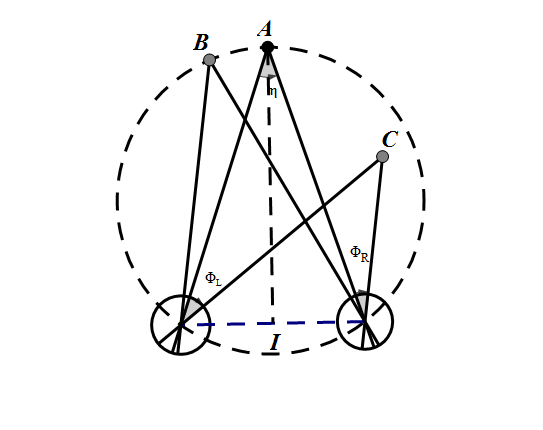
\includegraphics[width=0.4\textwidth]{chap2/horopter.png}}
  \hspace{1in}
  \subfigure[当前双目视界的定义 \supercite{howarth2011geometric}]{
    \label{fig:newdef:b} %% label for second subfigure
    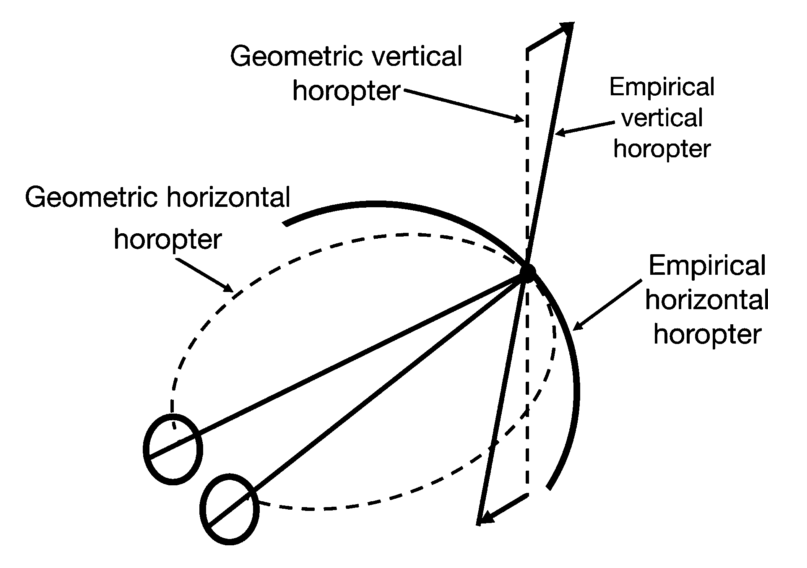
\includegraphics[width=0.4\textwidth]{chap2/modfiedhoropter.png}}
  \bicaption[fig:horopterdefinition]{双目视界的两种定义方式,图a是以前的球面模型截面,图b是最近研究结果定义的几何模型}{双目视界的几何定义}{Fig}{The geometry definition of binocular horopter}
\end{figure}
利用球面建立的双目视界的几何模型可以很好地说明视差角的概念,但是近年来新的研究成果表明,人眼双目视界并不是球面,而是由水平视界和竖直视界组成的综合体。在水平方向上表现为椭球面的一部分,在竖直方向上是一条与水平面呈现夹角的线段----水平面上方远离眼睛,水平面下方靠近眼睛。Howarth \parencite{howarth2011geometric}给出了这种双目视界的定义方法,如图\ref{fig:newdef:b}所示\parencite{zhu20143d}:

进一步地,该研究还表明,双目水平视界的局部曲率很小,竖直视界的夹角也不大。正是这个原因,即使当前主流电视屏幕都是平的,且竖直摆放,也不会造成我们观看的不便,因为电视处于双目视界的局部位置,在水平方向和竖直方向都可以近似认为是“平坦竖直的”。

基于上述分析,我们知道日常生活中电视摆放的位置实质上近似于双目视界所在的位置,因此,在观看3D电视时,由于双目视界在局部范围内曲率很小,所以通常认为电视屏幕就是双目视界,即零视差平面。结合前面对视差角的定义,本文给出在观看3D电视时视差角的计算方法。

主流的3D电视支持多种格式的3D图像与视频,但是最终处理的结果都是左眼看到左图,右眼看到右图,左右眼所看到的图像在水平方向显示差异,这样就会产生水平视差,从而使用户产生出立体感。整个过程实际上模拟了人眼视觉系统。如图\ref{fig:disparitydifinition}所示,假设眼睛$L$,$R$与显示器的中心$C$位于同一水平面,且双眼关于屏幕中垂线对称,$A$,$B$为同一点在左、右图上的位置,当$A$在$B$的左边时,左右眼视线交于屏幕内部,产生入屏效果;当$A$在$B$的右边时,左右眼视线相交于屏幕外面,产生出屏效果;$A$和$B$重合时,双眼视线交于屏幕上,此时所看的场景与2D图像效果相同。3D电视中图像中一点的视差的定义为右眼所看到的该点的横坐标与左眼看到的匹配点横坐标之差,即:
\begin{figure}[!htp]
  \centering
  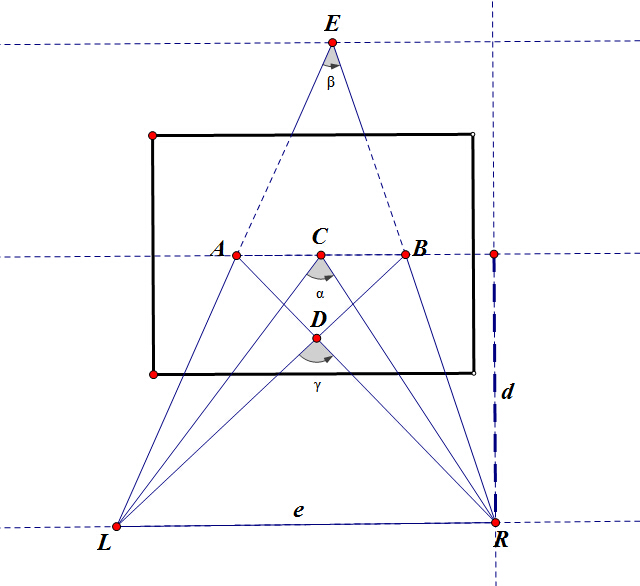
\includegraphics[width=0.5\textwidth]{chap2/disparitydifinition.jpg}
  \bicaption[fig:disparitydifinition]{立体电视下的视差角定义}{立体电视下的视差角定义}{Fig}{Disparity definition under 3DTV watching circumstances}
\end{figure}
\begin{equation}
\label{chap2:eq:disparitypixel}
D = {x_r} - {x_l}
\end{equation}

这种表示方法可以说明此时场景的出入屏关系,但是不能用来直接描述人眼的立体感知,这是因为人的立体感知与观看环境和人眼双目距相关。因此,视觉中精确的视差信息以视差角来表示。由于屏幕近似于双目视界,因此,这里的视差角可以通过对公式\ref{eq:disparitydefine1}进行变形得到,用$\theta $表示视差角,则视差角可以定义为左右眼视线在屏幕上的汇聚角与左右眼视线的实际汇聚角之差。如图\ref{fig:disparitydifinition}所示:
出屏时视差角:
\begin{equation}
\label{eq:posdisparity}
\theta  = \alpha  - \gamma 
\end{equation}
入屏时
\begin{equation}
\label{eq:negdisparity}
\theta  = \alpha  - \beta 
\end{equation}
这样我们得到了在观看3D电视时视差角的定义。

\section{眼动数据中的视差角计算方法}
\label{sec:caldisparity}
\ref{sec:stereodisparity}概述了观看3D电视时的视差角计算方法,是一种理想状态下的定义。眼动数据的收集也是在观看3D电视时收集的,但是眼动数据来自真实测量,其与理想状况存在以下区别:
\begin{itemize}[noitemsep,topsep=0pt,parsep=0pt,partopsep=0pt]
\item 人眼双目距不再以均值65mm取代,眼动仪会计算出当前测试者的真实双目瞳距;
\item 左右眼视线和屏幕的交点不一定在同一水平线,可能存在竖直视差;
\item 双目关于屏幕中轴未必对称,特别是采用非侵入式眼动仪采集眼动数据时,肯定存在这样的问题。
\end{itemize}

针对以上差异,不同的眼动仪有不同的处理方式。对于头部固定的眼动仪,$Wang$等\parencite{wang2014online}提出了一种简单地处理方法。由于眼睛位置相对稳定,且头部固定支架和屏幕的位置可以摆置得近似对称,同时也能保证眼睛到屏幕的距离为3倍屏高。所以,只需要测量双目距,并利用左右视线与屏幕交点纵坐标的均值代替两个交点的纵坐标,即若$A({x_a},{y_a})$,$B({x_b},{y_b})$为视线与屏幕的交点,且${y_a} \ne {y_b}$,则修正后的交点为$A'({x_a},({y_a} + {y_b})/2)$,$B'({x_b},({y_a} + {y_b})/2)$,这样,所有的条件满足\ref{sec:stereodisparity}的计算方法的要求,利用方程\ref{eq:posdisparity}和\ref{eq:negdisparity}的具体实现方程\ref{eq:chap4:disparitycal}便可以求得结果。

对于头部不固定的眼动仪,如本论文研究所使用的眼动仪,前述处理方法引入的误差会比较大。幸运的是,眼动数据包含了同一坐标系下眼睛位置的坐标以及在屏幕上注视点的坐标,很容易得到视线的向量,这样就可以得到视线的汇聚角,同时用两个交点的平均位置估计中央眼视线在屏幕上的交点,可以算出视线在屏幕上的汇聚角。此时采用方程\ref{eq:posdisparity}或\ref{eq:negdisparity}可以求得视差角,更具体的,如图\ref{fig:realsightline:a}所示,用$O_1$,$O_2$表示双目位置,$G_l$,$G_r$表示左右眼在屏幕上的注视点,则$G_c=(G_l+G_r)/2$是人眼在屏幕上的汇聚点的估计。此时视差角可以定义为:
\begin{equation}
\label{eq:disparityofeyetrackdata}
\theta = \arccos(\frac{{\overrightarrow {{O_1}{G_c}}  \bullet \overrightarrow {{O_2}{G_c}} }}{{\left| {{O_1}{G_c}}
 \right|\left| {{O_2}{G_c}} \right|}}) - \arccos (\frac{{\overrightarrow {{O_1}{G_l}}
  \bullet \overrightarrow {{O_2}{G_r}} }}{{\left| {{O_1}{G_l}} \right|\left| {{O_2}{G_r}}
  \right|}}).
\end{equation}
更一般地,屏幕不同区域视差角的定义方法示意图如图\ref{fig:eyetrackdisparitydifinition:b}。
\begin{figure}
  \centering
  \subfigure[眼动数据测量的实际视线与注视点]{
    \label{fig:realsightline:a} %% label for first subfigure
    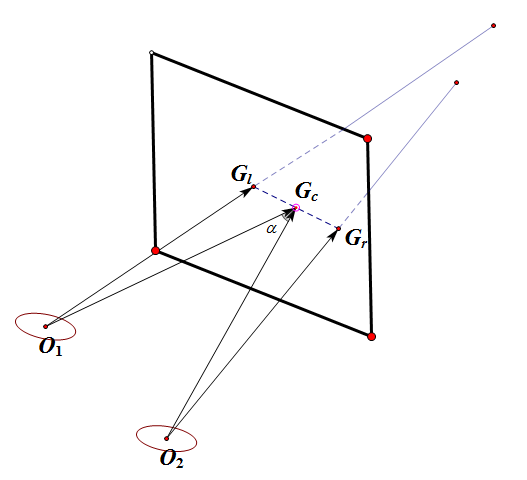
\includegraphics[width=0.4\textwidth]{chap2/angularbysightline.png}}
  \hspace{1in}
  \subfigure[屏幕不同区域的视差角定义方法]{
    \label{fig:eyetrackdisparitydifinition:b} %% label for second subfigure
    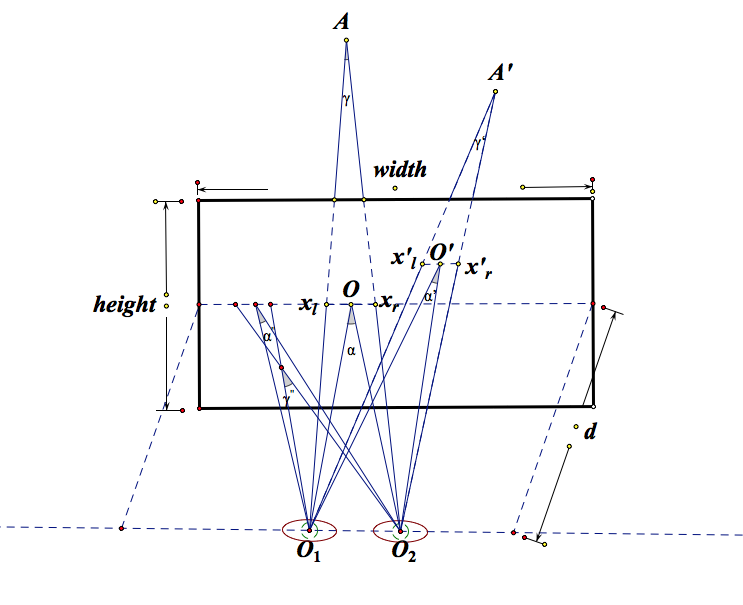
\includegraphics[width=0.4\textwidth]{chap2/eyetrackdisparitydefinition.png}}
  \bicaption[fig:eyetrackrealdisparity]{眼动数据的视差角标示图}{眼动数据的视差角标示图}{Fig}{Disparity angular definition of Eyetracking Data}
\end{figure}

我们对此稍作说明,如图\ref{fig:realsightline:a},眼动数据会告诉我们双目位置${O_1}$,${O_2}$ 以及屏幕上的注视点$G_l$,$G_r$,此时可以求得左右视线汇聚角$\gamma$,同时利用两个注视点的平均位置$O$,估计视线在屏幕上的汇聚角$\alpha$,这样视差角为$\alpha$与$\gamma$之差。需要说明的是,屏幕的双目视界的特性保证了这种方法不同区域屏幕汇聚角的计算是等价的。

\section{总结}
\label{sec:conclusionchapter2}
本章描述了人眼视觉系统的生理过程。单目视觉系统是光线进入眼睛的第一步,这里负责控制进入眼睛的光的量,同时可以对亮度和色度等特征进行预处理,还完成了光信号到电信号的转化以及电信号的传递。单目肌肉是眼睛运动的动力来源,它使得眼睛可以自由转动以适应各种深度的物体。正是这样的生理特性,构成了眼动仪的生理学基础。双目视觉系统是形成立体视觉的核心,主要由位于大脑皮层V1区域和纹状皮层的简单细胞和复杂细胞完成。此过程是进入视觉系统的信号进行编码的过程,生理学在双目视觉过程的研究成果,是近年来基于人眼注视模型的图像质量评价方法兴起的重要支撑。同时,由于眼睛运动的过程是双目系统处理信息的反馈过程,这也为眼动仪等注视模型的建立奠定了基础。

本文还讨论了双目视觉中特别重要的因素-----视差,在这个过程中,我们发现,摆放在适当位置(一般三倍屏高)的3D显示器实际上是双目视界的一种近似,这从理论上解决了将电视屏幕设为零视差平面的合理性。对于视差角的计算,本文讨论了理想状况与实际情况的联系与区别,结合双目视界的特性,本文给出了眼动数据的视差角计算方法,为后续的眼动数据的应用做好准备。
